% !TeX spellcheck = pl_PL

\rozdzial

%%%%%%%%%%%%%%%%%%%%%%%%%%%%%%%%%%%%%%%%%%%%%%%%%%%%%%%%%%%%%%%%%%%%%%%
\section{Ustawienia}
\label{ustawienia}

\begin{figure}[htb]
	\centering
	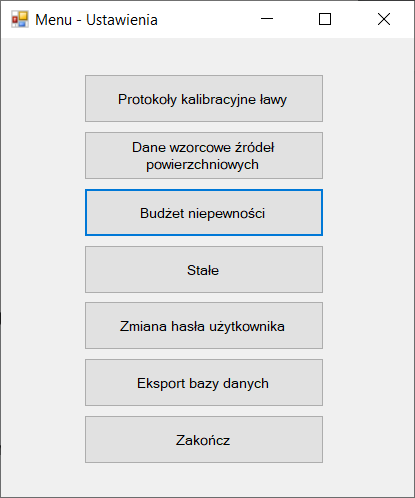
\includegraphics{obrazki/Ustawienia/menu_ustawienia.png}
	\caption{Menu ustawienia}
	\label{menuUstawienia}
\end{figure}

\subsection{Budżet niepewności}
\label{budzet}

W tym oknie (rys. \ref{budzetNiepewnosci}) można zobaczyć aktualny budżet niepewności związany z wyznaczeniem całkowitej niepewności pomiaru przy wzorcowaniu przyrządu dozymetrycznego promieniowaniem gamma.

Znaczenie poszczególnych symboli:
\begin{itemize}
	\item \textbf{$N_{R}$} - współczynnik kalibracji przyrządu referencyjnego
	\item \textbf{$M_{R}$} - wskazanie przyrządu referencyjnego
	\item \textbf{$k_{pr}$} - współczynnik korekcyjny odchylenia ciśnienia od jego wartości odniesienia
	\item \textbf{$k_{T}$} - współczynnik korekcyjny odchylenia temperatury od jej wartości odniesienia
	\item \textbf{$k_{t}$} - współczynnik korekcyjny na rozpad źródła Cs-137
	\item \textbf{$k_{r}$} - współczynnik korekcyjny na odchylenie odległości przyrządu referencyjnego od wartości nominalnej
	\item \textbf{$k_{d}$} - współczynnik korekcyjny na odchylenie odległości przyrządu dozymetrycznego od wartości nominalnej
\end{itemize}

Wartość całkowitej względnej niepewności standardowej wylicza się według poniższego wzoru (\ref{budzetwzor}):

\begin{equation}
	\label{budzetwzor}
	w = \sqrt{{w^2(N_{R})}+{w^2(M_{R})}+{w^2(k_{pr})}+{w^2(k_{T})}+{w^2(k_{t})}+{w^2(k_{r})}+{w^2(k_{d})}}
\end{equation}

gdzie:
\begin{itemize}
	\item \textbf{$w(N_{R})$} - względna niepewność standardowa współczynnika kalibracji przyrządu referencyjnego
	\item \textbf{$w(M_{R})$} - względna niepewność standardowa wskazania przyrządu referencyjnego
	\item \textbf{$w(k_{pr})$} - względna niepewność standardowa współczynnika korekcyjnego odchylenia ciśnienia od jego wartości odniesienia
	\item \textbf{$w(k_{T})$} - względna niepewność standardowa współczynnika korekcyjnego odchylenia temperatury od jej wartości odniesienia
	\item \textbf{$w(k_{t})$} - względna niepewność standardowa współczynnika korekcyjnego na rozpad źródła Cs-137
	\item \textbf{$w(k_{r})$} - względna niepewność standardowa współczynnika korekcyjnego na odchylenie odległości przyrządu referencyjnego od wartości nominalnej
	\item \textbf{$w(k_{d})$} - względna niepewność standardowa współczynnika korekcyjnego na odchylenie odległości przyrządu dozymetrycznego od wartości nominalnej
\end{itemize}

\begin{figure}[htb]
	\centering
	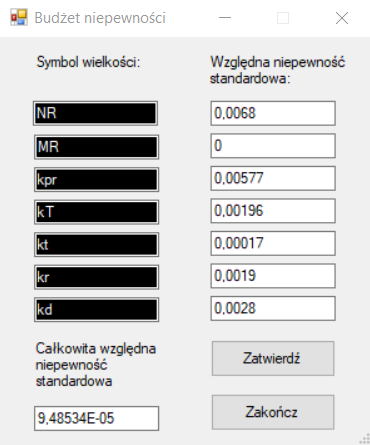
\includegraphics{obrazki/Ustawienia/budzet_niepewnosci.png}
	\caption{Okno budżetu niepewności.}
	\label{budzetNiepewnosci}
\end{figure}

Zmiany w wartościach poszczególnych wielkości można wprowadzić poprzez zmienienie ich w odpowiednim polu, a następnie zatwierdzenie zmian za pomocą przycisku \textbf{"Zatwierdź"}.

\subsection{Protokoły kalibracyjne ławy}
\label{protokoly_kal_lawy}

Ta część programu umożliwia zarządzanie protokołami kalibracyjnymi ławy. Tabela (rys. \ref{protokolyKalLawy}) przedstawia wartości wzorcowe mocy kermy wraz z niepewnościami względnymi dla poszczególnych kombinacji odległości i numeru źródła. Za pomocą strzałek przy polu \textbf{"Numer protokołu"} możemy przechodzić pomiędzy poszczególnymi protokołami. Pole \textbf{"Data"} podaje datę pomiarów dla danego protokołu kalibracyjnego. Zarówno datę jak i konkretne wartości pól w tabeli można edytować (klikając dwukrotnie na wybranym polu). Należy jednak wprowadzone poprawki zatwierdzić przyciskiem \textbf{"Zatwierdź poprawki"}.

\textbf{TIP:} Nowe dane wzorcowe należy wprowadzić możliwie szybko, po każdym ich przygotowaniu. Zaleca się porównanie starych aktualnie stosowanych danych z nowo uzyskanymi w celu minimalizacji prawdopodobieństwa błędu.

\begin{figure}[htb]
	\centering
	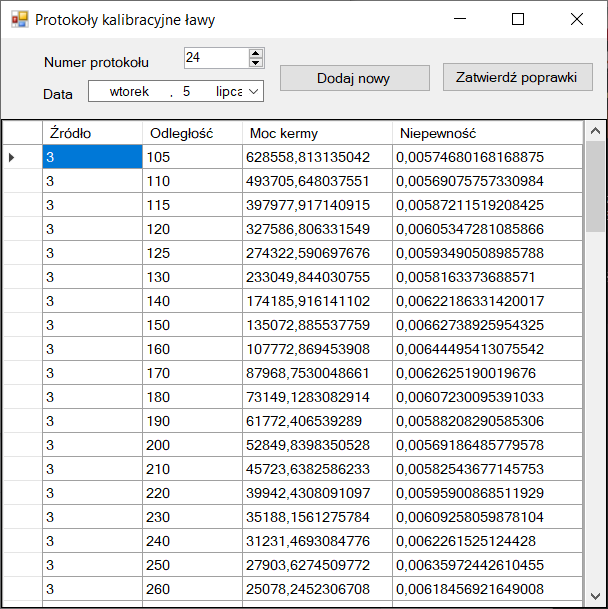
\includegraphics{obrazki/Ustawienia/protokoly_kalibracyjne_lawy.png}
	\caption{Okno do zarządzania protokołami kalibracyjnymi ławy.}
	\label{protokolyKalLawy}
\end{figure}

Przejście do okna umożliwiającego wprowadzenie nowego protokołu kalibracyjnego następuje poprzez przycisk \textbf{"Dodaj nowy"}. Otwiera się okno analogiczne do poprzedniego rys. \ref{protokolyKalLawyDodaj}. Nowy protokół można dodać zarówno ręcznie jak i zaimportować go z odpowiednio przygotowanego pliku Microsoft Excel. W obu przypadkach pierwszym krokiem jest wybranie daty, mówiącej kiedy wykonane zostały pomiary wartości wzorcowych. Następnie można albo ręcznie przekopiować wartości wzorcowe do tabeli, bądź też użyć przycisku \textbf{"Zaimportuj z Excela"}. W tym drugim przypadku otwiera się okno managera plików, w którym należy wybrać przygotowany wcześniej plik. 

\textbf{TIP:} Aby plik MS Excel dobrze się wczytał powinien mieć 4 kolumny, w których kolejno będą się znajdować: numer źródła, odległość, moc dawki i niepewność względna.

\begin{figure}[htb]
	\centering
	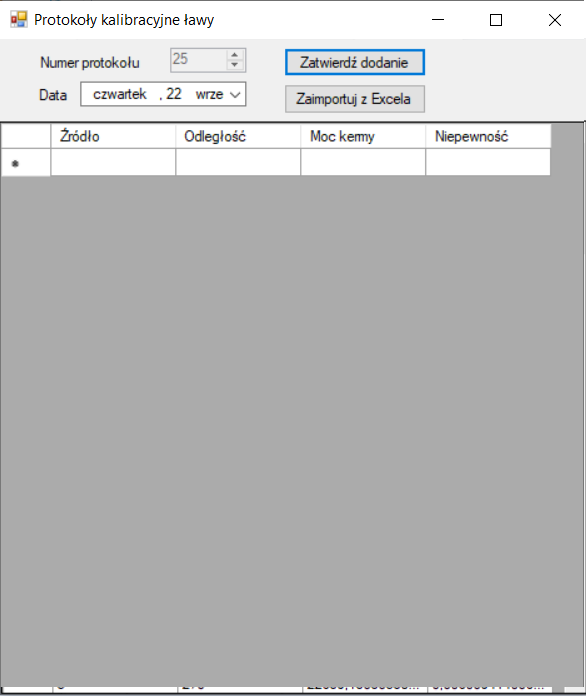
\includegraphics{obrazki/Ustawienia/protokoly_kalibracyjne_lawy_dodawanie.png}
	\caption{Dodawanie nowego protokołu kalibracyjnego.}
	\label{protokolyKalLawyDodaj}
\end{figure}

\subsection{Wzorcowanie źródeł}
\label{wzor_zrodel}

Okno \ref{wzorcowanieZrodelPowierzchniowych} przedstawia dane kalibracyjne źródeł powierzchniowych. Dane zawarte w tabeli można edytować klikając na wybraną komórkę. Jako, że w kolumnie "Źródło" znajduje się "ID" źródła, to aby ułatwić użytkownikowi identyfikację źródła edycja pól tej kolumny następuje poprzez wybór odpowiedniej nazwy źródła z listy rozwijanej \textbf{"Wybór numeru źródła"}. Podobnie edycja daty wymaga wybrania jej w kalendarzu \textbf{"Wybór daty wzorcowania"}. Dokonane zmiany należy zatwierdzić klikając przycisk \textbf{"Zatwierdź poprawki"}. 

\textbf{TIP:} Nowe dane kalibracyjne należy wprowadzić poprzez dodanie nowego wiersza w tabeli, a nie edycję już istniejącego (również dla źródeł już uwzględnionych w tabeli).

Dodanie nowych danych kalibracyjnych następuje po naciśnięciu przycisku \textbf{"Dodaj"}. Wciśnięcie tego przycisku powoduje przejście do nowego okna z taką samą, ale pustą tabelą. Tutaj klikając na odpowiednie pola możemy uzupełnić dane z nowego świadectwa kalibracyjnego. Analogicznie jak w przypadku edycji danych, źródło wprowadzamy poprzez wybór jego nazwy na liście rozwijanej \textbf{"Wybór numeru źródła"}, a datę wzorcowania w kalendarzu ("\textbf{"Wybór daty wzorcowania"}). Wprowadzone dane zatwierdzamy klikając przycisk \textbf{"Zatwierdź dodanie"}.

\textbf{TIP:} Każdorazowo po otrzymaniu nowego świadectwa wzorcowania źródła powierzchniowego należy wprowadzić aktualne dane do bazy.

\begin{figure}[htb]
	\centering
	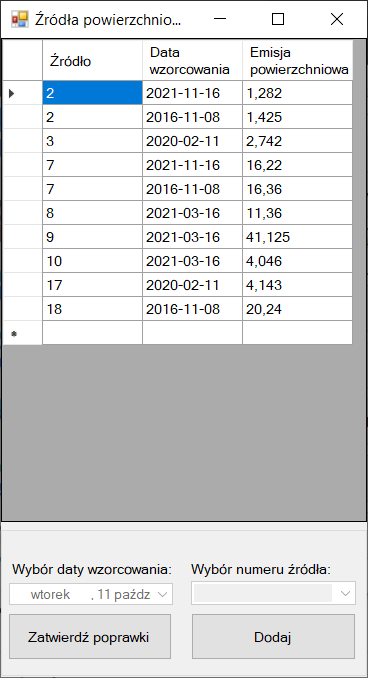
\includegraphics{obrazki/Ustawienia/wzorcowanie_zrodel_powierzchniowych.png}
	\caption{Dane kalibracyjne źródeł powierzchniowych.}
	\label{wzorcowanieZrodelPowierzchniowych}
\end{figure}

\subsection{Stałe}
\label{stale}

W tym oknie wyświetlone są wszystkie stałe, które są niezbędne do prawidłowego funkcjonowania programu. W szczególności do obliczeń współczynników kalibracyjnych i niepewności, a nie zostały ujęte w innych miejscach: budżecie niepewności (patrz \ref{budzet}), protokołach kalibracyjnych źródła gamma (patrz \ref{protokoly_kal_lawy}) lub źródeł powierzchniowych (patrz \ref{wzor_zrodel}). Tabela podaje parametr oraz aktualnie stosowaną jego wartość. 
Aby zmienić wartość jakiegoś parametru, należy wpisać ją w odpowiednią komórkę tabeli, a następnie zatwierdzić zmianę przyciskiem \textbf{"Aktualizuj"}.

\textbf{TIP:} Przy każdej zmianie procedury WZOR-1 lub WZOR-2 należy upewnić się, że wartości w tabeli \textbf{"Stałe"} są aktualne.

\begin{figure}[htb]
	\centering
	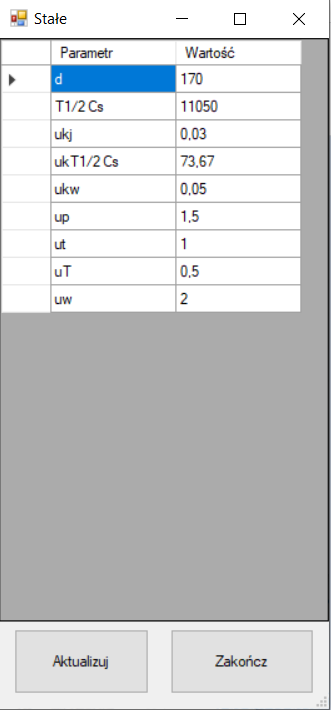
\includegraphics{obrazki/Ustawienia/stale.png}
	\caption{Okno ze stałymi.}
	\label{staleOkno}
\end{figure}

\subsection{Zmiana hasła}
\label{zmiana_hasla}

W tym oknie użytkownik może zmienić swoje hasło do programu na nowe (rys. \ref{zmianaHasla}). W polach należy wpisać odpowiednio swoje aktualne hasło, nowe hasło i powtórnie nowe hasło. Następnie zatwierdzić przyciskiem \textbf{"OK"}. Hasło nie powinno być krótsze niż 8 znaków, musi zawierać co najmniej jedną literę i co najmniej jedną cyfrę.
	
\textbf{TIP:} Hasło należy zapamiętać i regularnie zmieniać (np. raz w miesiącu).

\begin{figure}[htb]
	\centering
	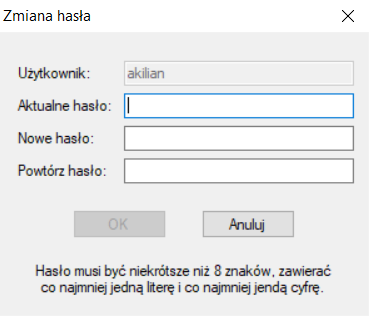
\includegraphics{obrazki/Ustawienia/zmiana_hasla.png}
	\caption{Okno zmiany hasła użytkownika.}
	\label{zmianaHasla}
\end{figure}

\subsection{Eksportuj}
\label{eksport}

Przycisk eksportuj umożliwia wyeksportowanie pliku bazy danych (w formacie Microsoft Access). Po wciśnięciu przycisku należy wybrać i zatwierdzić ścieżkę do zapisu. Pojawi się okno, w którym należy ustawić hasło do wyeksportowanej bazy danych (rys. \ref{zmianaHaslaBazyEksportowanej}).
Hasło nie powinno być krótsze niż 8 znaków, musi zawierać co najmniej jedną literę i co najmniej jedną cyfrę.

\textbf{TIP:} Hasło należy zapamiętać.

\begin{figure}[htb]
	\centering
	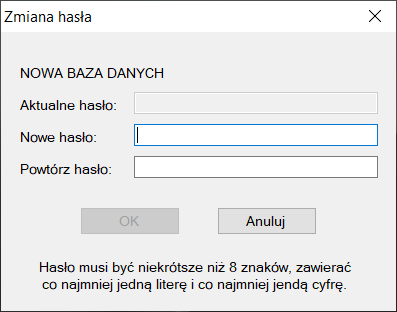
\includegraphics{obrazki/Ustawienia/zmiana_hasla_bazy.PNG}
	\caption{Okno ustawienia hasła do eksportowanej bazy danych.}
	\label{zmianaHaslaBazyEksportowanej}
\end{figure}